%% ------------------------------------------------------------------------- %%
\chapter{Study pipeline}
\label{cap:study-methodology}

The main objective of this work is to study and compare the impact of selected hyperparameters in different models trained on different datasets, using the LightGBM gradient boosting algorithm. Each "type" of dataset will be aggregated in different categories using the values of aggregated characteristics of the dataset itself (e.g. number of features, number of instances), this can be checked on Section \ref{dataset-aggregated-statistics}.

In the following sections an overview about the methodology and experimental setup is given, explaining the datasets, the hyperparameters chosen and its distributions, pipeline for testing and the tools used in each step.

%% ------------------------------------------------------------------------- %%
\section{Tools}

All of the study pipeline and analysis is done using Python 3.6. Besides the commonly used data science tools (\textit{numpy, pandas, matplotlib, seaborn}) the most important packages used are:

\begin{itemize}
    \item \textbf{fklearn}: Functional machine learning library, developed by Nubank and built on top of \code{scikit-learn} and main machine learning implementations, e.g. the \code{LightGBM}; It has very useful abstractions, used in this study to build a pipeline of multiple learners and applying the same evaluation function;
    \item \textbf{toolz}: Add more functional programming functionality into python, trying to follow the principles of composability, purity and laziness.
    \item \textbf{scikit-learn}: The most widely used machine learning library for python;
    \item \textbf{pingouin}: Statistical package, mainly used for ANOVA tests and Levene's test for homoscedasticity. More details about it can be found in \cite{Vallat2018};
    \item \textbf{scipy}: Scientific computing package, the most used module was \code{scipy.stats} for statistical tests on the experiment results;
    \item \textbf{scikit-posthoc}: Library from the \textit{scikit} environment, which provides post hoc tests for pairwise multiple comparisons that are usually performed in statistical data analysis to assess the differences between group levels if a statistically significant result of ANOVA (or the equivalent nonparametric test) test has been obtained, more details in \cite{Terpilowski2019}.

\end{itemize}

%% ------------------------------------------------------------------------- %%
\section{OpenML Datasets}

The OpenML project has an online service to ``(...) share, organize
and reuse data, code and experiments. Following best practices observed in other sciences, OpenML allows collaborations to scale effortlessly and rewards scientists for sharing
their data more openly'' (\cite{Vanschoren:2014:ONS:2641190.2641198}).

In the research of previous studies for this work, it was noted that OpenML was being used in different scientific studies related to machine learning; A specific subset of datasets was used in \cite{probst2018tunability} to conduct a large-scale benchmarking to measure hyperparameter tunability, and it was also used in \cite{couronne2018random} as a benchmark platform for automatically retrieving datasets and comparing different machine learning algorithms.

OpenML provides a python API package for automatically retrieving datasets, tasks, submit customized runs and obtaining OpenML flows (a description of a personalized machine learning task). In this study, the datasets used are retrieved using the python API, and filtered according to some personalized rules, which are:

\begin{enumerate}
    \item  \textbf{\code{classes} = 2}, the study consists of analyzing binary classification problems;
    \item  \textbf{\code{min\_num\_features} = 3}, the dataset must have at least 3 features;
    \item  \textbf{\code{min\_num\_instances} = 1000}, the dataset must have at least $1000$ instances (data points);
    \item  \textbf{\code{max\_num\_instances} = 5000000}, the dataset must have at most $5$ million data points (provided just as an upper bound, no dataset used had more then $2$ million instances);
    \item  \textbf{\code{max\_nan\_percentage} = 20\%}, LightGBM has built-in support for missing values (\textit{NaNs}), but the datasets are filtered to have at most 20\% of its total number of rows with some missing values, for more meaningful data and simplicity.
\end{enumerate}

\begin{figure}[!h]
    \centering
    \includegraphics[width=1\textwidth]{openml_eda1.png} 
    \caption{Number of datasets after filtering is close to 400}
    \label{fig:openml-eda1}
\end{figure}

After all these filters, the number of valid datasets for the experiment would be close to 400 (figure \ref{fig:openml-eda1}), in theory. However, a lot of datasets could not be opened by the python API due to a variety of errors, mostly related to Attribute-Relation File Format (ARFF) in python. This brought the number of possible datasets to experiment close to $200$, but since each hyperparameter experiment takes a long time to run (favoring more hyperparameter space covered over the number of datasets, check \ref{subsec:hp-tree}), the final number of datasets analyzed in this study is 70.


Each dataset retrieved by the OpenML API has a dataset id (\code{did}) related to it, along with very useful metadata related to it, as it can be seen in Figure \ref{fig:openml-eda3}. With a simple exploratory analysis of the datasets it was observed a great number of datasets with high number of categorical variables, and usually high number of features too. Datasets with only textual data as features were also removed from the study, along with features not explicitly indicated as a categorical feature by the API.

\begin{figure}[!h]
    \centering
    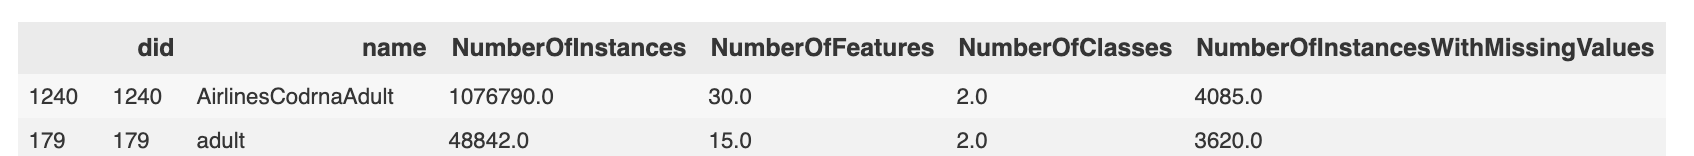
\includegraphics[width=1\textwidth]{openml_eda3.png} 
    \caption{Example of dataset information from OpenML}
    \label{fig:openml-eda3}
\end{figure}

Analyzing the number of instances in the subset of datasets used in this study, it can be seen that most of the datasets have a relatively small number of instances, but a portion of them have more than $300000$ data points, in hope to cover more data-heavy models (\ref{fig:openml-eda2}).

\begin{figure}[!h]
    \centering
    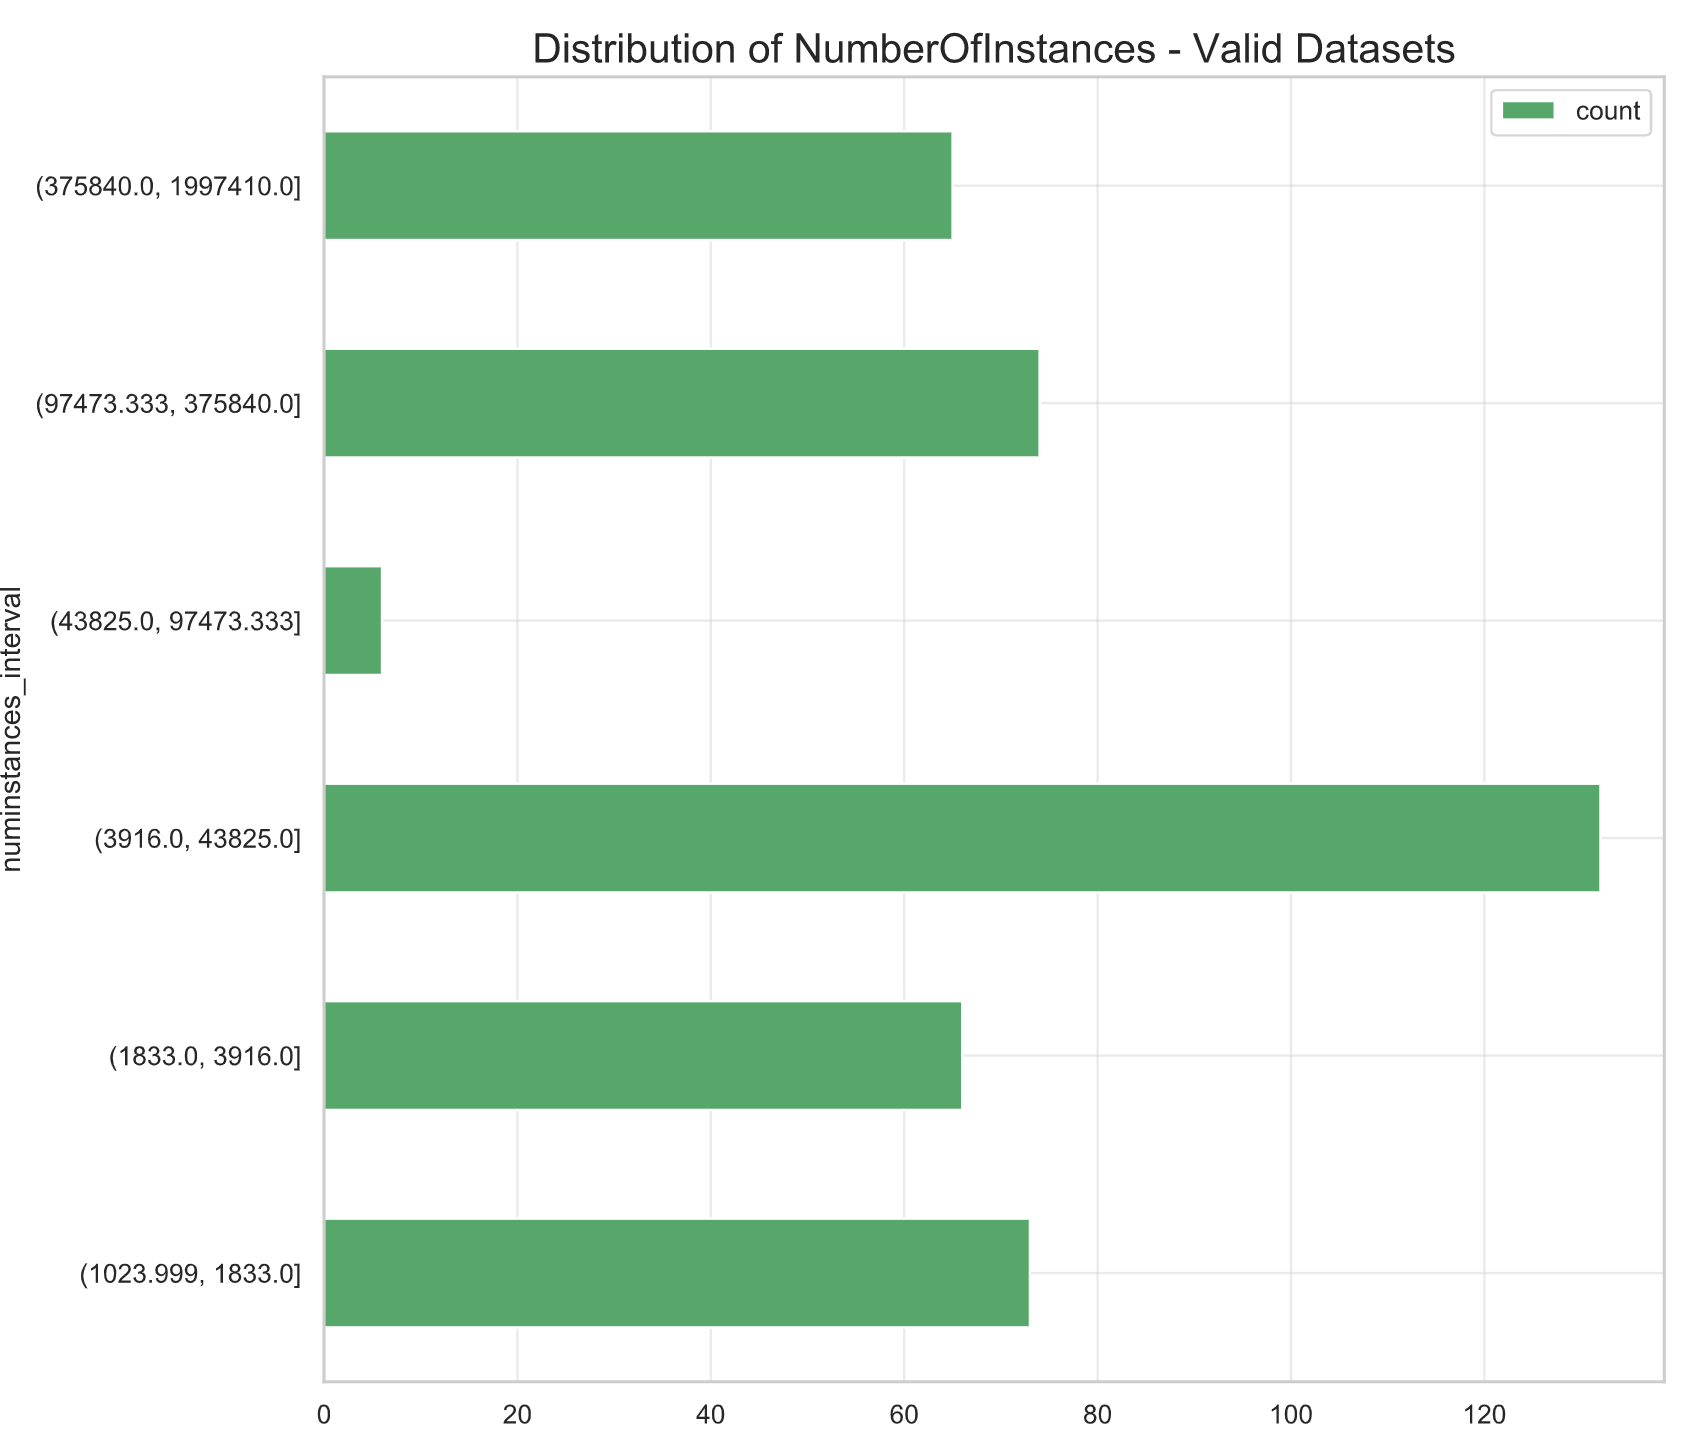
\includegraphics[width=.7\textwidth]{openml_eda2.png} 
    \caption{Number of data points distribution}
    \label{fig:openml-eda2}
\end{figure}

\newpage

\subsection{Data Cleaning}

In this study there are only two data cleaning steps, with the objective to keep the cleaned dataset as close as possible to the original to not interfere with the experiment results.
\begin{enumerate}
    \item The OpenML provides an attribute describing which of the features in the dataset are the categorical features; In the dataset building process, the type of each variable is identified (using \textit{pandas-profiling} package), and from each identified feature as "categorical", remove all that aren't explicitly declared by the OpenML attributes;
    \item The data in each OpenML dataset doesn't follow a specific pattern, e.g. some datasets represent the \textbf{target} variable as a string (\textit{'y'} and \textit{'n'}), some are represented in floating point, Boolean, etc. In the experiment pipeline, the \textbf{target} is converted to an integer, if possible. If not, the \textbf{target} is encoded using a \textit{label encoder}.
\end{enumerate}

%% ------------------------------------------------------------------------- %%
\section{Descriptive dataset statistics}
\label{dataset-aggregated-statistics}

To analyze subgroups of datasets and categorize each one of them, multiple statistics related to the structure of the dataset is calculated before any machine learning model is trained. Before the training process, the granularity of these statistics are feature-wise, which are then further aggregated in the result analysis step.

\textbf{Categorical features} are known to cause a \textit{prediction shift} in traditional gradient boosting models, as demonstrated in \cite{prokhorenkova2018catboost}. This shift is identified as a special kind of target leakage, which can also be caused in a preprocessing step of categorical features when using target statistics (e.g. using the target/mean encoding technique)\footnote{To fix this kind of problem in a dataset with many categorical features a new boosting algorithm was developed by \cite{dorogush2018catboost} called \textbf{Catboost}.}. As noted in the mentioned paper, LightGBM converts categorical features to gradient statistics at each step of the boosting process (as explained in Section \ref{lightgbm-explanation}), which result in some information loss. To categorize datasets with relation to categorical features, in this work the following statistics related to categorical variables are calculated:

\begin{itemize}
    \item \textbf{cardinality}, is the number of unique categorical values of a given feature;
    \item \textbf{variance}, is  a simple measure of variability of a specific categorical feature.
    Let $|top_{j}|$ be the number of occurrences of the most frequent category in feature $j$, i.e. the column $\xmat_{:, j}$. Then, this metric is defined as the inverse of the ratio of occurrences of the most frequent category:

    $$categorical\_variability=1 - \frac{|top_{j}|}{|\xmat_{:, j}|}$$

    As an example, if 90\% of the values of a given feature is the same, then the categorical variability of the said feature is $0.1$.
\end{itemize}

For \textbf{numeric features}, the main specific statistic calculated is the sample \textbf{skewness} of each feature. Skewness is a degree of distortion of a distribution, and in this study it's calculated using the unbiased adjusted Fisher–Pearson standardized moment coefficient from \textit{pandas}. The skewness is also trying to measure the variability of the numeric features, and is used in the clustering of each dataset as a feature.

The pipeline also calculates other useful statistics for each feature, like the percentiles, number of NaNs, infinite values, mean, median, etc. They're useful in the exploratory step, but are not used when clustering the datasets in the result analysis step.

%% ------------------------------------------------------------------------- %%
\section{Hyperparameter space}
\label{sec:hyperparam-space}

In section \ref{gbm-hyperparams} it's explained the basic hyperparameters used in LightGBM's gradient boosting algorithm. In this section the \textit{hyperparameter space}\footnote{In model tuning, the \textit{hyperparameter space} is the set of all the values each hyperparameter can assume in the tuning process.} of this study is explained, along with a simple overview of the hypothesis behind each distribution choice, related to LightGBM default hyperparameters and dataset size.  Let $D_i$ denote the number of instances of the $i$-th dataset, i.e. the total number of $\supervised$ pairs for the $i$-th dataset. 

\subsection{Hyperparameters tree}
\label{subsec:hp-tree}

The intention is to train multiple models changing the hyperparameters values, and calculate the metrics (explained in Section \ref{classification-metrics}) for each combination of hyperparameter. In this study three hyperparameters are studied: \textbf{\code{max\_depth}}, \textbf{\code{learning\_rate}} and \textbf{\code{num\_estimators}}.

In this study, the  \textit{hyperparameter space} also represents all valid hyperparameters values to run for the datasets, and is a function of $D_i$. The hyperparameter space is represented as a special tree, where each new leaf of the tree takes its parent node and generate new leafs based on a new hyperparameters. Let $LR_i$, $NE_i$ and $MD_i$ denote the sets of possible hyperparameter values for learning rate, number of estimators and maximum depth, respectively. Let $S_i$ be the set of all hyperparameter sets, i.e. $S_i = \{LR_i, NE_i, MD_i\}$, and $\mathcal{P}(s_i)$ the \textit{power set} of $S_i$. The number of values to test for each hyperparameter is denoted with the numbers $N_{LR}$, $N_{NE}$, $N_{MD}$: e.g. if $N_{LR} = 4$ it means $4$ values of learning rate will be generated (equivalent to say $|LR_i| = 4$).

For a given tree depth $k$, the hyperparameter set to be explored at that depth is defined using the rule in equation \ref{eq:hyperparam-tree}, where $\prod$ is the cartesian product operator.

\begin{equation}\label{eq:hyperparam-tree}
    C_k = \Big\{\prod_{X \in Q} X : Q \in \mathcal{P}(s_i), |Q| = k\Big\}
\end{equation}


\begin{figure}[!h]
    \centering
    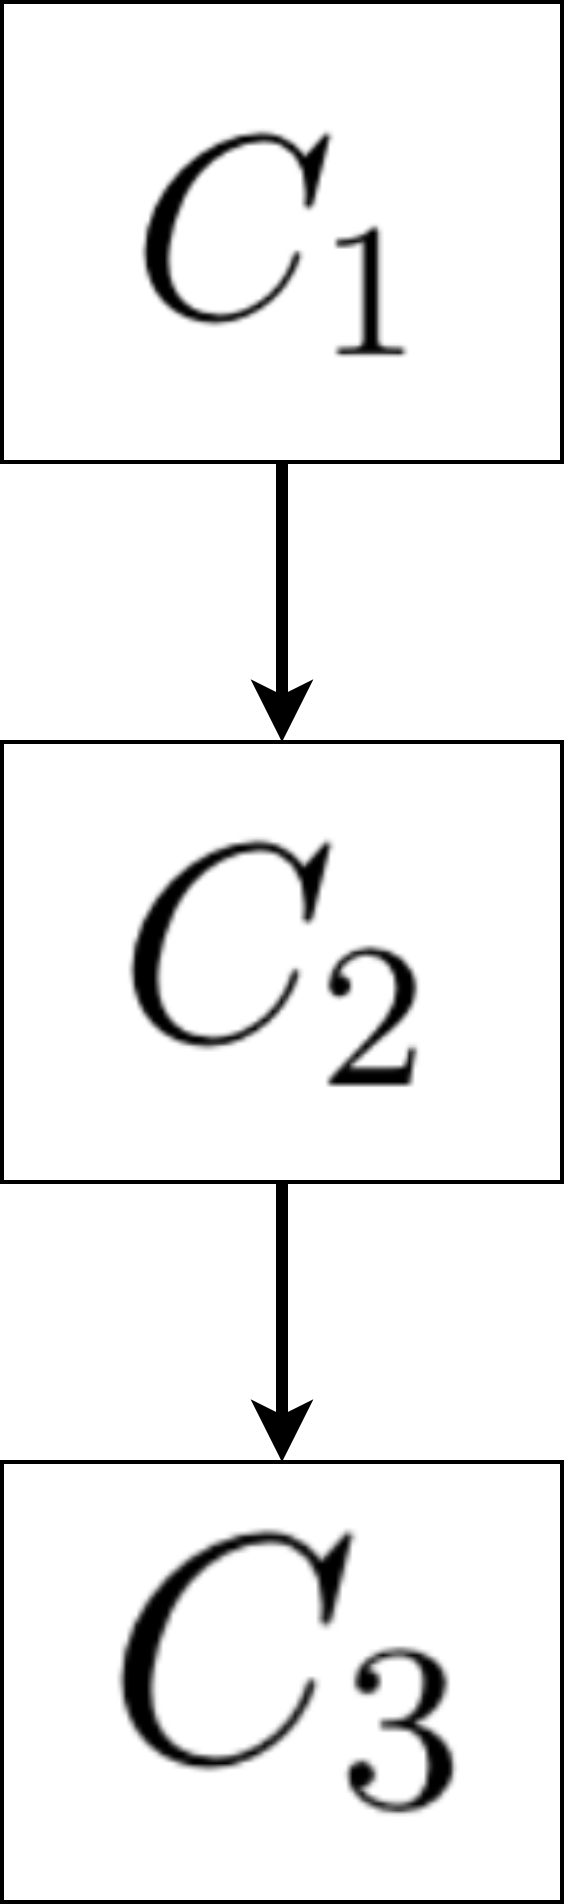
\includegraphics[height=.3\textwidth]{hp_tree.png} 
    \caption{Hyperparameter tree}
    \label{fig:hp-tree}
\end{figure}

The hyperparameter tree of this study, represented in Figure \ref{fig:hp-tree}, is then defined as different cartesian products of all valid $k$ combinations. Since there are three hyperparameters being changed, the maximum is $k=3$, and the final space is the union of all cartesian products combinations:

$$Hspace_i = C_1 \cup C_2 \cup C_3$$

This structure is generalizable for any number of hyperparameters, and it was designed this way to measure hyperparameter impact depending on the number of combinations. E.g. it is expected that changing multiple hyperparameters at the same time has a bigger impact on the model performance than changing just one. Each level of the hyperparameter tree represents a "combination effect", i.e. the experiment can measure, for multiple combinations of hyperparameters, which combination effect provides the biggest impact on the metrics (for better or worse) compared with the other combinations.

As an example, consider the three sets of hyperparameters below:

$$LR = \{0.1, 0.2\}$$
$$NE = \{1, 2\}$$
$$MD = \{10, 20\}$$

Then each leaf of the hyperparameter tree will be:

$$C_1 = \Big\{\{0.1, 0.2\}, \{1, 2\}, \{10, 20\}\Big\}$$

\begin{align*}
    C_2 = \Big\{\{(0.1, 1), (0.1, 2), (0.2, 1), (0.2, 2)\}, \\
            \{(0.1, 10), (0.1, 20), (0.2, 10), (0.2, 20)\}, \\
            \{(1, 10), (1, 20), (2, 10), (2, 20)\}\Big\}
\end{align*}

\begin{align*}
    C_3 = \Big\{\{(0.1, 1, 10), (0.1, 1, 20), (0.1, 2, 10), (0.1, 2, 20), \\
    (0.2, 1, 10), (0.2, 1, 20), (0.2, 2, 10), (0.2, 2, 20)\}\Big\}
\end{align*}

It can be observed that the number of hyperparameters in each tree node increase multiplicatively with the number of initial hyperparameters and the number of layers $k$ in the hyperparameter tree, and it's one of the reasons why the experiment may take a long time to run depending on the dataset. This was the chosen configuration of the experiment since the objective is not to perform a model tuning, but rather to measure the "magnitude" of the effects in performance metrics. Better strategies could be used for model tuning like Grid Search, Random Search or Bayesian Optimization, as it's stated in \cite{probst2018tunability}.

\subsection{Maximum Depth}
\label{subsec:max-depth}
The maximum depth is the hyperparameter that controls the maximum possible depth each boosting tree can have. As explained in Section \ref{gbm-hyperparams}, LightGBM default behavior is to grow the trees leaf-wise, having an unbound maximum depth, but the structure being controlled by the number of leaves in the tree. Max depth is a way to apply a constraint on the function space, i.e. the possible hypothesis the learning algorithm can use, and is commonly optimized in classical decision trees for pruning. 

Since gradient boosting harness the power of weak learners by combining them, usually the depth of a single tree isn't as deep as a traditional single classification tree. For example, in XGBoost the default value for max depth is $6$, while in the \textit{rpart} package in R (single decision trees) the default max depth is $30$. Even though in gradient boosting the max depth can be used to constraint the model, one can overfit in the data given a high enough number of boosting iterations : this can be seen as an ``overfit relationship'' between \code{max\_depth} and \code{num\_estimators}. For this reason, when defining the maximum depth or which values of it to optimize in a model tuning step there's isn't a clear rule to choose an optimal value. 

In this study, the tested maximum depth values are always the same, independent on the dataset size:

$$MD_i = \{3, 4, ..., N_{MD} + 3\}$$

In the experiments $N_{MD} = 20$, so each dataset is run using max depth from $3$ to $22$. The intuition behind these values is to neither test with very big depth values, nor very small depth for a weak learner in gradient boosting. The \code{num\_leaves} parameter is automatically set to be $\min(2^{max\_depth} - 1, 2^{15})$, because this way the number of leaves will not influence too much the results when changing the maximum depth and at the same time the number of nodes in each boosting tree will not grow unbound when training with \code{max\_depth} $\geq 16$.

\subsection{Learning rate}

The learning rate distribution is simple, and it depends only on the dataset size $D_i$. In XGBoost the default value of learning rate (also called \textit{eta}) is $0.3$ and in LightGBM it's $0.1$, which is also the default learning rate for \textit{scikit-learn} implementation of gradient boosting. Since in the OpenML datasets the dataset sizes aren't too similar (see Figure \ref{fig:openml-eda2}), the distribution of learning rate values to generate is a simple function starting from $0.01$ for small datasets, changing based on the dataset size.

\textbf{Premise:} Start with a learning rate value between $0.01$ for small datasets, and a multiple of $0.1$ for bigger datasets (a rule was defined by dividing $D_i$ by $10000$). Then, experiment with bigger and smaller values of learning rate around the "middle" value.

First it is defined a "middle" learning rate value $\psi_i$ (defined in equation \ref{eq:lr-eq1}). Then the values are generated as a list using $N_{LR}$, with the intention to generate a symmetric pattern of learning rates (the total length of each "side" of the learning rate list is described in \ref{eq:lr-eq2}).

\begin{equation}
    \psi_i = \max\Big(0.01, 0.1 \times \max(1, \frac{D_i}{10000})\Big)
    \label{eq:lr-eq1}
\end{equation}

\begin{equation}
    \kappa_i = \cdot \max\left(\lfloor\frac{N_{LR}}{2}\rfloor, 2\right)
    \label{eq:lr-eq2}
\end{equation}

The symmetric pattern and the final $LR_i$ are generated following the rule described in equation \ref{eq:lr-eq3}. By changing the maximum length $N_{LR}$ and the dataset size $D_i$, one can see the learning rate distribution behavior: In Figure \ref{fig:hyperparam-lr1} all the $D_i$ from the study are categorized in percentiles, and depending on the length ($N_{LR}$) a given distribution of learning rate values $LR_i$ is shown.

\begin{equation}
    LR_i = \Big\{\frac{\psi_i}{\kappa_i}, \frac{\psi_i}{\kappa_i - 1}, \frac{\psi_i}{\kappa_i - 2}, ..., \text{\Large $\psi_i$}, ..., (\kappa_i - 2)\cdot\psi_i, (\kappa_i - 1)\cdot\psi_i, \kappa_i\cdot\psi_i\Big\}
    \label{eq:lr-eq3}
\end{equation}

In this study $5$ unique learning rates are generated.

\begin{figure}[!h]
    \centering
    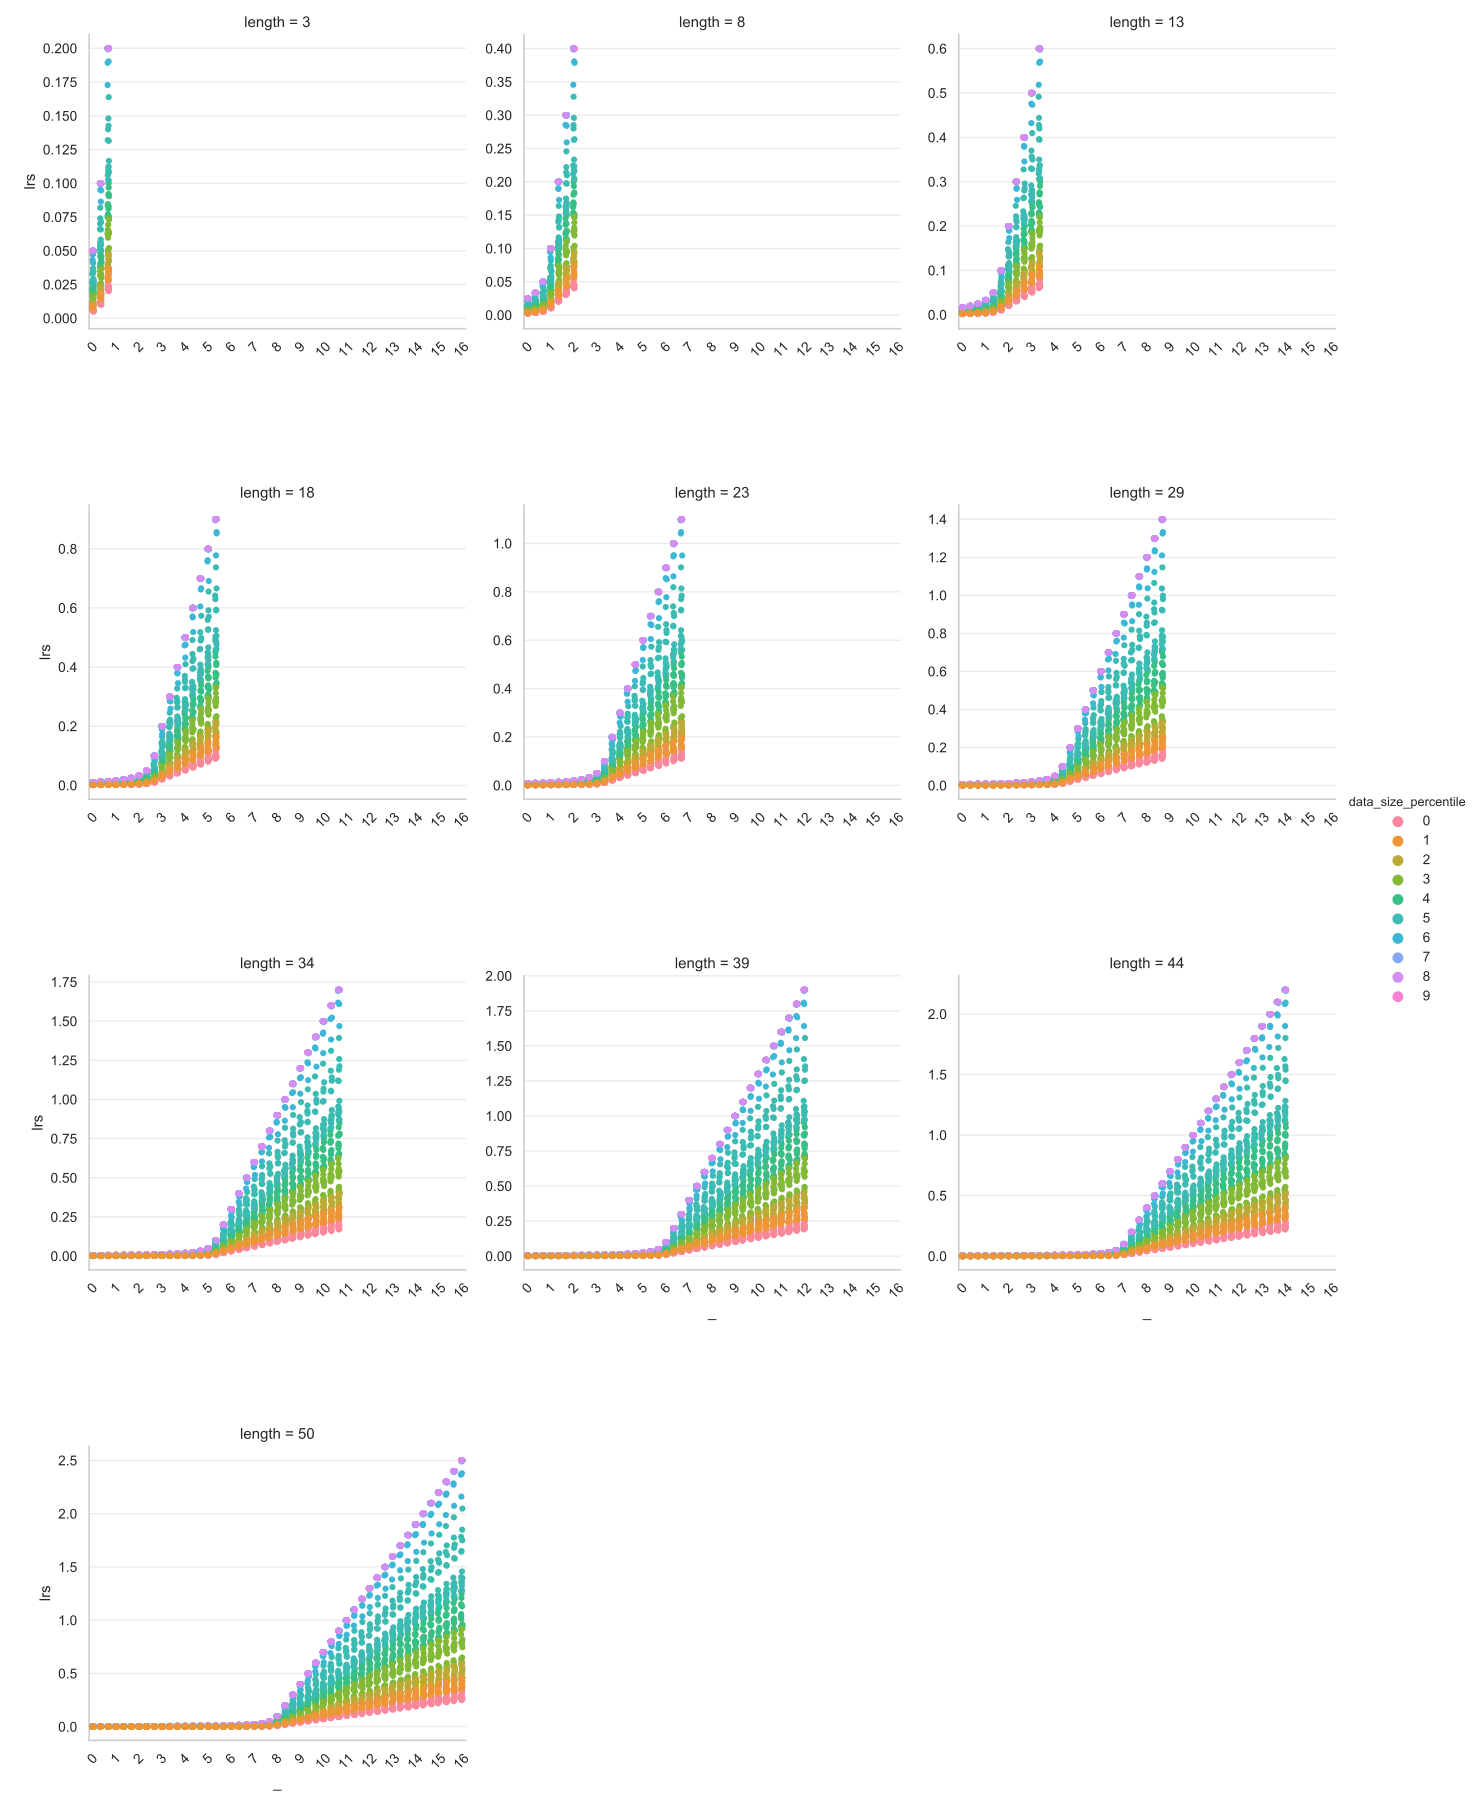
\includegraphics[width=1\textwidth]{learning_rate_binary.png} 
    \caption{Learning rate distribution, changing $D_i$ and $N_{LR}$. Bigger dataset sizes generate higher learning rates.}
    \label{fig:hyperparam-lr1}
\end{figure}

\subsection{Number of Estimators}

Both in XGBoost (\code{XGBClassifier}) and LightGBM the default value for the number of estimators is set to $100$. The optimal number of boosting iterations can be influenced by the dataset size: by fixing other hyperparameters, a model of a dataset with very few data points can converge much faster (i.e. in few boosting iterations) than a dataset with 10 times its size. Since in the study the intention is to test different boosting iterations, and the actual distribution ideally depends on $D_i$, first the maximum value of estimators a given dataset can have is defined, and then  multiple values of \code{num\_estimators} are generated. 

The definition of this function is a little arbitrary, but the objective is to cover different values and tie together the $D_i$ of the dataset. Using maximum values of $400$ estimators for small datasets and $1700$ for big datasets, along with the definitions of \textit{small} and \textit{big} datasets being $D_i\leq10000$ and $D_i>300000$ respectively, a linear function is then defined to calculate the maximum value to be assigned. After defining the constants in equation \ref{eq:num-est-1} the rule for the max value of \code{num\_estimators} is defined in equation \ref{eq:num-est-2}.

\begin{equation}
    a = \frac{1700 - 400}{300000 - 10000}, \text{ }b = 400 - a
    \label{eq:num-est-1}
\end{equation}
\begin{equation}
    max_{ne}(D_i) = \begin{cases}
        400 \text{ if } D_i \leq 10000 \\
        1700 \text{ if } D_i > 300000 \\
        a \cdot D_i + b
    \end{cases}
    \label{eq:num-est-2}
\end{equation}

The final list of number of estimators generated is then a linear interpolation starting at $min_{ne}(D_i) = \min(\frac{D_i}{4}, 50)$ to $max_{ne}(D_i)$, in evenly spaced steps (equation \ref{eq:hyperparam-ne-step}). An example of multiple $NE_i$ distributions is shown in Figure \ref{fig:hyperparam-ne1} for different $D_i$ values, but with a fixed length $N_{NE} = 20$.

$$step = \frac{\Big(max_{ne}(D_i) - min_{ne}(D_i)\Big)}{N_{NE} - 1}$$
\begin{equation}
    NE_i = \Big\{\lfloor min_{ne}(D_i) \rfloor,\lfloor min_{ne}(D_i) + step \rfloor,\lfloor min_{ne}(D_i) + 2\cdot step \rfloor, ... ,\lfloor max_{ne}(D_i)\rfloor\Big\}
    \label{eq:hyperparam-ne-step}
\end{equation}

\begin{figure}[!h]
    \centering
    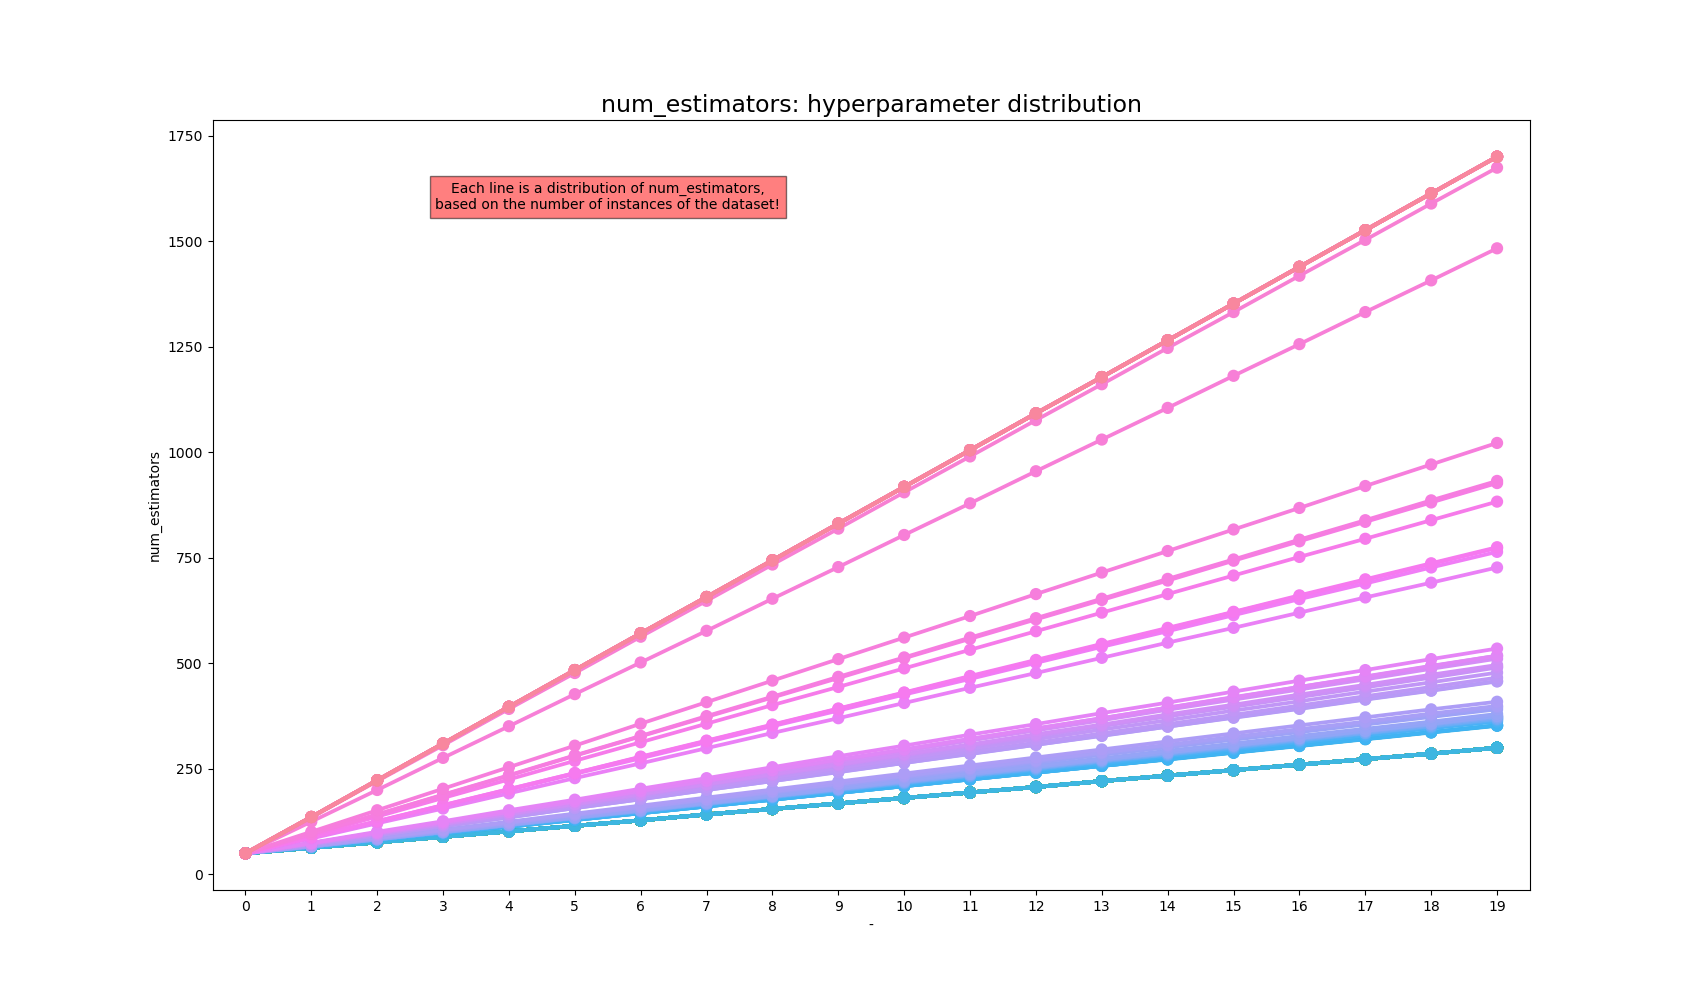
\includegraphics[width=1\textwidth]{num_estimators_binary.png} 
    \caption{Number of estimators distribution - changing $D_i$, for a fixed $N_{NE} = 20$. Bigger dataset sizes generate higher \textit{num\_estimators} values.}
    \label{fig:hyperparam-ne1}
\end{figure}

\newpage
\section{Final experiment pipeline}

For each dataset considered in this study a pipeline is built for it, following the sequence:

\begin{enumerate}
    \item Calculate the descriptive statistics for the dataset (see \ref{dataset-aggregated-statistics});
    \item Build the hyperparameter space $Hspace_i$;
    \item Split the dataset into train and test set;
    \item Build evaluators for each studied metric;
    \item Train a LightGBM model for each hyperparameter value $\in Hspace_i$, and evaluate it on the train and test set;
    \item Save logs.
\end{enumerate}

The train test split strategy chosen for all datasets is a random split with train size being 70\% of the data points and 30\% for test (\textbf{70/30}). Given a dataset, the split is fixed, i.e. the train and test is the same in all trained models.

\subsection{Label Encoding}

As stated in LightGBM's documentation, the library has a built-in support for categorical features, which uses a specific method from \cite{fisher1958grouping}. However, in order to make the study more general, it was decided to not use this specific feature of LightGBM. When categorical features are detected, a \textbf{label encoding} technique is used on the categorical values of the dataset. The label encoding is just a numeric encoding of the categorical features, i.e. each categorical value is mapped to an integer number. 
